\section{Linearizion}

\subsection{Find equilibrium point}

Find the fix point with $$x=y=z=\phi=\theta=\psi=0$$

If the system is filled out with these parameters a much simpler set of equations is obtained:

\begin{eqnarray}
\dot{x}=v_x \\
\dot{y}=v_y \\
\dot{z}=v_z \\
\dot{v_x}=-\frac{k \ d}{m}v_x \\
\dot{v_y}=-\frac{k \ d}{m}v_y \\
\dot{v_z}=-\frac{k \ d}{m}v_z -g + \frac{K \ C_m}{m}(v_1^2+v_2^2+v_4^2+v_4^2)\\
\dot{\phi}=w_x \\
\dot{\theta}=w_y \\
\dot{\psi}=w_z \\
\dot{w_x}=\frac{L \cdot k \cdot C_m}{I_{xx}}(v_1^2 - v_3^2) - \frac{I_{yy}-I_{zz}}{I_{xx}} w_y  w_z \\
\dot{w_y}=\frac{L \cdot k \cdot C_m}{I_{xx}}(v_2^2 - v_4^2) - \frac{I_{zz}-I_{xx}}{I_{yy}} w_y  w_z\\
\dot{w_z}=\frac{b \cdot C_m}{I_{yy}}(v_1^2-v_2^2+v_3^2-v_4^2) - \frac{I_{xx}-I_{yy}}{I_{zz}}w_y  w_z
\end{eqnarray}

Its very clear from the that $v_x,v_y,x_z,w_x,w_y$ and $w_z$ are zero ,the remaining equations are set equal to zero :

\begin{eqnarray}
\dot{v_z}= -g + \frac{K \ C_m}{m}(v_1^2+v_2^2+v_4^2+v_4^2) =0\\
\dot{w_x}=\frac{L \cdot k \cdot C_m}{I_{xx}}(v_1^2 - v_3^2) =0 \\
\dot{w_y}=\frac{L \cdot k \cdot C_m}{I_{xx}}(v_2^2 - v_4^2) =0\\
\dot{w_z}=\frac{b \cdot C_m}{I_{yy}}(v_1^2-v_2^2+v_3^2-v_4^2) =0
\end{eqnarray}

simplify even further:

\begin{eqnarray}
g =  \frac{K \ C_m}{m}(v_1^2+v_2^2+v_4^2+v_4^2)\\
v_1^2 - v_3^2 =0 \\
v_2^2 - v_4^2 =0\\
v_1^2-v_2^2+v_3^2-v_4^2 =0
\end{eqnarray}

This means that
\begin{eqnarray}
v_1^2 = v_3^2 \\
v_2^2 = v_4^2 \\
\end{eqnarray}

combine this with the last equation:

\begin{equation}
v_1^2=v_2^2=v_3^2=v_4^2
\end{equation}

This is to be expected as the motors should all be running at the same speed to Hoover. The speed at which these motors need to rotate depends on the gravity which is the last equation $$g =  \frac{K \ C_m}{m}(v_1^2+v_2^2+v_4^2+v_4^2) \\$$ As all the voltages are exactly the same this becomes: $$\frac{m \cdot g}{K \cdot C_m \cdot 4}=   v_i^2 = u_i \\$$ with $i=1...4$

and: $$v_1^2+v_2^2+v_3^2+v_4^2=\frac{m \cdot g}{K \cdot C_m}$$ 

\subsection{Define linear model}

The lineare model is of the form $$\triangle \dot{x}=A\triangle x + B\triangle u $$ $$ \triangle y=C\triangle x$$

The matrix is the Jacobian related to x and matrix B is the Jacobian related to u both evaluated in the equilibrium point.

$$x=[x \ y \ z \ v_x \ v_y \ v_z \ \phi \ \theta \ \psi w_x w_y w_z]  $$
$$x_{equilibrium} = [0\ 0\ 0\ 0\ 0\ 0\ 0\ 0\ 0\ 0\ 0\ 0]$$

$$
u_{equilibrium} =
 [\frac{m \cdot g}{K \cdot C_m \cdot 4} \frac{m \cdot g}{K \cdot C_m \cdot 4} \frac{m \cdot g}{K \cdot C_m \cdot 4} \frac{m \cdot g}{K \cdot C_m \cdot 4}] 
$$

$$
A(x_{equilibrium}) =
\begin{bmatrix}
0 & 0 & 0 & 1 & 0 & 0 & 0 & 0 & 0 & 0 & 0 & 0 \\
0 & 0 & 0 & 0 & 1 & 0 & 0 & 0 & 0 & 0 & 0 & 0 \\
0 & 0 & 0 & 0 & 0 & 1 & 0 & 0 & 0 & 0 & 0 & 0 \\

0 & 0 & 0 & -\frac{k_d}{m} & 0 & 0 & 0 & g & 0 & 0 & 0 & 0 \\
0 & 0 & 0 & 0 & -\frac{k_d}{m} & 0 & -g & 0 & 0 & 0 & 0 & 0 \\
0 & 0 & 0 & 0 & 0 & -\frac{k_d}{m} & 0 & 0 & 0 & 0 & 0 & 0 \\

0 & 0 & 0 & 0 & 0 & 0 & 0 & 0 & 0 & 1 & 0 & 0 \\
0 & 0 & 0 & 0 & 0 & 0 & 0 & 0 & 0 & 0 & 1 & 0 \\
0 & 0 & 0 & 0 & 0 & 0 & 0 & 0 & 0 & 0 & 0 & 1 \\

0 & 0 & 0 & 0 & 0 & 0 & 0 & 0 & 0 & 0 & 0 & 0 \\
0 & 0 & 0 & 0 & 0 & 0 & 0 & 0 & 0 & 0 & 0 & 0 \\
0 & 0 & 0 & 0 & 0 & 0 & 0 & 0 & 0 & 0 & 0 & 0
\end{bmatrix}
$$



$$
u = [u_1 \ u_2 \ u_3 \ u_4] = [v_1^2 \ v_2^2 \ v_3^2 \ v_4^2 ]
$$

$$
B(u_{equilibrium}) = 
\begin{bmatrix}
0 & 0 & 0 & 0 \\ %x
0 & 0 & 0 & 0 \\ %y
0 & 0 & 0 & 0 \\ %z

0 & 0 & 0 & 0 \\ %vx dot
0 & 0 & 0 & 0 \\ %vy dot
\frac{k c_m}{m} & \frac{k c_m}{m} & \frac{k c_m}{m} & \frac{k c_m}{m} \\

0 & 0 & 0 & 0 \\
0 & 0 & 0 & 0 \\
0 & 0 & 0 & 0 \\

\frac{L K c_m }{I_{xx}} & 0 & -\frac{L K c_m }{I_{xx}} & 0 \\
0 & \frac{L K c_m }{I_{yy}} & 0 & -\frac{L K c_m }{I_{yy}} \\
\frac{b c_m }{I_{zz}} & -\frac{b c_m }{I_{zz}} & \frac{b c_m }{I_{zz}} & -\frac{b c_m }{I_{zz}}\\
\end{bmatrix}
$$

\subsection{Numerical matrices}
The simplest test of the linear model is to apply an step impulse to all motors at the same time. This should only affect the z-axis as can be seen on Figure~\ref{fig:test lin model}. As the equilibrium point take is the one with the quad copter hovering still on one location.
\subsection{Test Linear model}
\begin{figure}[H]
	\centering
	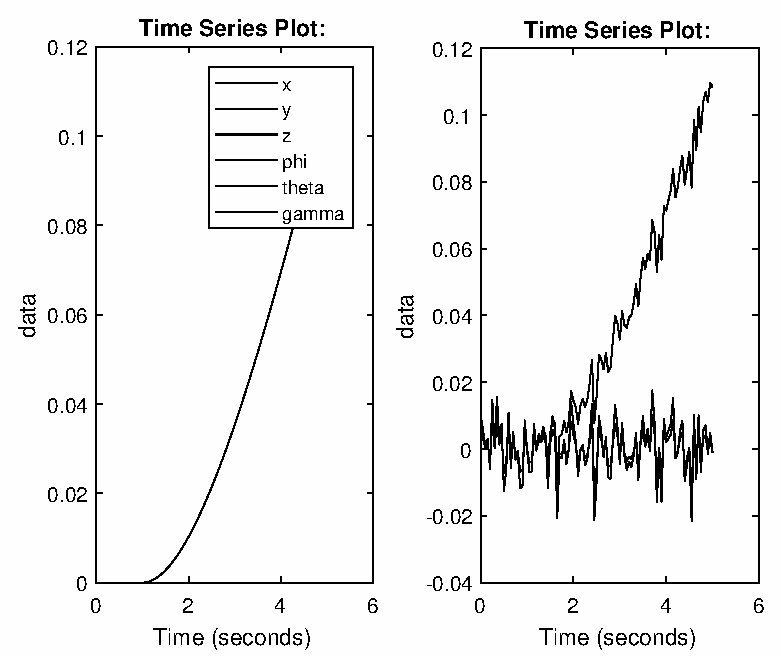
\includegraphics[width=7cm]{./img/lin_approx/step_all.eps}
	\caption{impulse to all engines, linear model on the left, non linear on the right}
	\label{fig:test lin model}
\end{figure}

